\documentclass[]{article}
\usepackage{amsmath} % flere matematikkommandoer
\usepackage{amssymb}
\usepackage[utf8]{inputenc} % æøå
\usepackage[T1]{fontenc} % mere æøå
\usepackage[danish]{babel} % orddeling
\usepackage{verbatim} % så man kan skrive ren tekst
\usepackage[all]{xy} % den sidste (avancerede) formel i dokumentet
\usepackage{graphicx}
\usepackage{listings}
\usepackage{algorithmic}
\usepackage{algorithm}

\begin{document}

\title{Hobe og Prioritetskøer}
\maketitle
{\setlength{\parindent}{0 cm}

\section*{Introduktion}

\textbf{Prioritetskøer}\\

En prioritetskø implementerer et set S med elemeter, som hver i sær er forbundet med en nøgle. Dannelse af prioritetskø er $O(lgN)$, og er somregel repræsenteret med en hobe (som et træ)\\

\textbf{Operationer på prioritetskøer} \\

\textbf{insert(S, x)} - indsætter et element x ind i et set $S$\\
\textbf{max(S)} - returnerer elementet med den største nøgle i et set $S$\\
\textbf{extract-max(S)} - returnerer elementet med den største nøgle i et set $S$ og fjerne det fra sættet efterflg.\\
\textbf{increase-key(S, x, k)} - Inkrementerer værdien af x's nøgle til værdien af k

\section*{Hobe}

Træet's rod er det første elemet (i = 1)\\
Forældre til en knude floor(i/2)\\
Venstre barn: (2i), højre barn: (2i + 1)\\
Max-heap: En knudes nøgle $\ge$ dens børns nøgle.\\
Min-heap: En knudes nøgle $\le$ dens børns nøgle.\\

\section*{Hobeoperationer}

\textbf{build-max-heap}: Producerer en max-heap fra et usorteret array\\
\textbf{max-heapify}: Retter en overtrædelse af hobeegenskaben i et deltræ's rod.\\
\textbf{insert}: Tilføjer et element til bunden af hoben, sammenligner med sin forældre indtil den er i korrekt rækkefølge.\\
\textbf{Delete}: Erstat roden af hoben med hobens sidste element. Kør nu max-heapify indtil de er i korrekt rækkefølge.

\newpage
\section*{Eksempel}
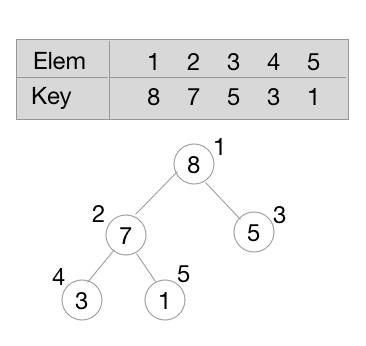
\includegraphics[width=10cm]{graphics/Heapsort Example.png}
\newpage

\section*{Bevis lower-bound}

Antag at alt andet en sammenligninger er gratis.

Enhver sammenligningssortering gør flg.

1. Find relative sammenligningsinformation mellem alle elementer.

2. Flyt elementerne til deres korrekte positioner.\\

Vi har et input $A[1..n]$, som bliver kørt på en sorteringsalgoritme C.

C tager en beslutning om at sammenligne elementerne $A[i]:A[j]$

Lad os sige at resultatet er $A[i] > A[j]$

Næst beslutter C at sammenligne elementerne $A[x] : A[y]$

Denne procedure gentages til der er nok information til at bestemme sorteringsrækkefølgen.\\

Nu bliver $A$ ændret og C køres igen $C(A)$

$A[i] : A[j]$, er ændret til $A[i] < A[j]$

Da C ikke kan se forskelligheden på det gamle og det nye A vil den's næste valg være det samme: $A[x] : A[y]$\\

Vi kan nu observere at hvis sekvensen af de tidligere valg og de tilhørende resultater er ens, vil C altid foretage det samme valg næste gang.

Hvis C nu biver kørt på alverdens input, vil der blive opbygget et træ med valg og resultater (Decision Tree)

Ud fra det kan vi se at der er $n! \le \# blade \le 2^h $

$h \ge lg(n!) = lg(n) + lg(n-1) + \dots $

$\ge lg(n) + \dots lg(n/2)$

$\ge (n/2) lg(n/2) = \Theta (nlgn)$

Konklussion er at i værste tilfælde er antallet af sammenligniger $= h = \Theta(nlgn)$
}
\end{document}